\maketitle
\setcounter{page}{1}
\tableofcontents
\newpage
\pagenumbering{arabic}
\section{Theorie}
Der Photoeffekt beschreibt die Auslösung von Elektronen aus Metalloberflächen
durch das Einwirken von Licht. Dabei spielt die Natur des Lichtes eine Rolle.
Einige Phänomene, wie Beugung und Interferenz, lassen auf eine Wellennatur
des Lichtes schließen, während zum Beispiel der Compton-Effekt oder eben der
Photoeffekt nicht mit dem Wellenmodell zu vereinbaren sind. Um dieses Dilemma zu lösen,
wird die Quantenelektrodynamik genutzt. Diese enthält das Korpuskel- und Wellenmodell
als Grenzfälle. Bei einer großen Anzahl von Photonen lässt sich das Wellenmodell gut verwenden,
bei allen Wechselwirkungen von Licht mit Materie das Korpuskelmodell. \\
\\
In Abbildung \ref{fig:1} ist der schematische Aufbau zur Untersuchung des Photoeffekts abgebildet.
\begin{figure}[h]
  \centering
  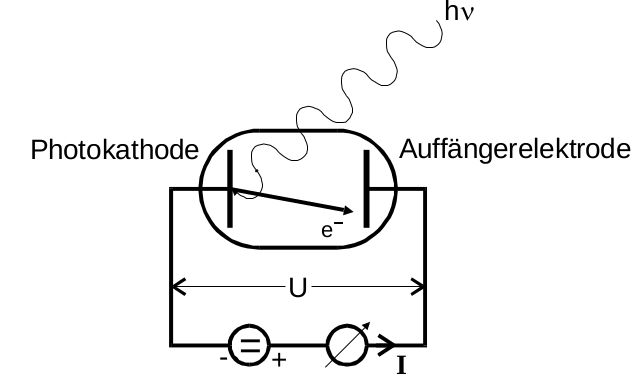
\includegraphics[scale=0.4]{aufbautheorie.png}
  \caption{Schema des Versuchsaufbaus zur Untersuchung des Photoeffekts.}
  \label{fig:1}
\end{figure}
Dabei fällt monochromatisches Licht in einer Vakuumröhre auf eine als Photokathode bezeichnete Elektrode.
Ihr gegenüber liegt eine Elektrode, die ein positives Potential gegenüber der anderen Elektrode besitzt.
Diese nennt man Auffängerelektrode. Folgende Ergebnisse lassen sich aus diesem Aufbau gewinnen:
\begin{itemize}
  \item Es besteht ein proportionaler Zusammenhang zwischen der Zahl der pro Zeiteinheit ausgelösten
  Elektronen und der Lichtintensität.
  \item Die Energie der ausgelösten Elektronen ist proportional zur Frequenz des einfallenden
  Lichts, aber unabhängig von der Intensität.
  \item Es existiert eine Grenzfrequenz, unterhalb jener kein Photoeffekt auftritt.
\end{itemize}
All diese Erkenntnisse widersprechen der Wellennatur des Lichts, so müsste auch bei rotem
(sehr langwelligem) Licht nach genügend langer Einstrahlung ein Photoeffekt auftreten, d.h es
gäbe keine Grenzfrequenz. Weiterhin
wären die Energie der Photoelektronen, also die Elektronen, die mittels Photonenbeschuss aus dem Metall
gelöst wurden, abhängig von der Lichtintensität. Nimmt man stattdessen das Korpuskelmodell als gegeben an,
dann lassen sich alle experimentellen Resultate auf theoretischer Basis bestätigen. Im Einzelnen bedeutet dies:
\begin{itemize}
  \item Monochromatisches Licht mit der Frequenz $\nu$ besteht aus sich gradlinig bewegenden Photonen,
  die alle die Energie $E = h \nu$ besitzen.
  \item Beim Aufprall auf ein Elektron überrägt ein Photon eine Energie auf jenes Elektron. Diese spaltet
  sich nach
  \begin{equation}
    h \nu = A_k + E_{\symup{kin}}
    \label{eqn:1}
  \end{equation}
  auf. Dabei ist $A_k$ die Austrittsarbeit, die nötig ist, damit das Elektron den Potentialtopf
  des Metallgitters verlassen kann und $E_{\symup{kin}}$ die kinetische Energie des Elektrons
  nach dem Stoß. Mit \eqref{eqn:1} folgt, dass im Fall $h\nu < A_k$ kein Photoeffekt auftreten kann.
  Somit lässt sich das Auftreten einer Grenfrequenz erklären.
  \item Die Lichtintensität verhält sich proportional zur Zahl der Photonen pro Zeit- und Raumwinkeleinheit.
\end{itemize}
Um die kinetische Energie der schnellsten Elektronen zu berechnen, wird die
Gegenfeldmethode\footnote{Näheres in Kapitel \ref{sec:aufbau}} verwendet. Dabei endet
der Elektronenfluss von Kathode zu Anode, falls
\begin{equation}
    \symup{e}_0 U_g = \frac{1}{2} \, \symup{m}_0 v_{\symup{max}}
    \label{eqn:2}
\end{equation}
gilt. Dabei ist $v_{\symup{max}}$ die Geschwindigkeit der schnellsten Elektronen
und $\symup{e}_0$ und $\symup{m}_0$ die Elementarladung bzw. die Ruhemasse des Elektrons.
Aus \eqref{eqn:1} und \eqref{eqn:2} folgt
\begin{equation}
    h \, \nu = \symup{e}_0 U_g +A_k \, .
    \label{eqn:3}
\end{equation}
Aus \eqref{eqn:3} lässt sich also das Verhältnis von Wirkungsquantum $h$ zu Elementarladung
$\symup{e}_0$ mithilfe einer Messreihe von $U$ in Anhängigkeit von $\nu$ bestimmen.

Im Versuch ergibt sich allerdings das Problem, dass der Photostrom nicht abrupt
bei $U = U_g$ abfällt, sondern wie in Abbildung \ref{fig:5} sich der Grenzspannung annähert.
\begin{figure}[h]
  \centering
  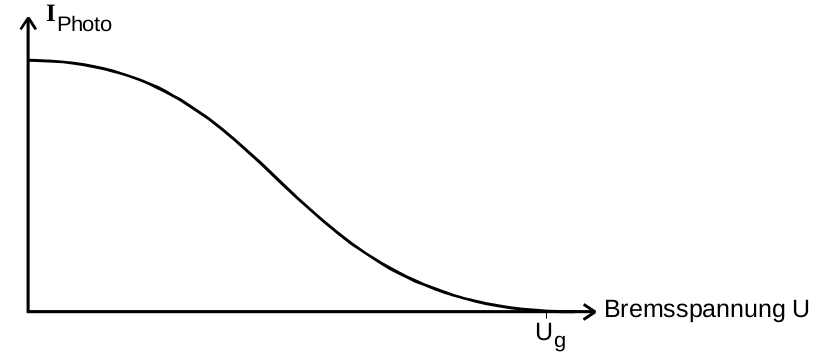
\includegraphics[scale=0.3]{photo.png}
  \caption{Der Photostrom in Abhängigkeit von der Bremsspannung.}
  \label{fig:5}
\end{figure}
Dies lässt sich dadurch erklären, dass die Elektronen, die durch die Photonen
ausgelöst werden, nicht alle die gleiche Energie besitzen, da schon die Elektronen
im Metall nicht alle monoenergetisch sind. Die Energieverteilung im Festkörper wird
durch die Fermi-Dirac Statistik festgelegt. Diese besagt, dass die Energie der Elektronen
zwischen 0 und der materialabhängigen Fermi-Energie $\xi$ variiert. Es lässt sich zeigen,
dass zwischen dem Photostrom und der Bremsspannung die Beziehung
\begin{equation*}
    I_{\symup{ph}} \approx U^2
\end{equation*}
gilt. \\
\\
Ein weiteres Problem ergibt sich, wenn die Austrittsarbeit der Anode $A_a$ sehr groß ist.
Falls also $A_k < h \, \nu < A_a$ gilt, dann ist zwar der Photoeffekt theoretisch möglich, aber
es tritt kein Photostrom auf, da die Energie der Elektronen nicht ausreicht, um die Austrittsarbeit
der Anode zu überwinden. Aus diesem Grund muss eine Beschleunigerspannung $U_b$ angelegt werden, damit
ein Photostrom auftritt. Dann gilt
\begin{equation*}
  h \, \nu + \symup{e}_0 U_b \geq A_a \, .
\end{equation*}

\section{Durchführung}
\subsection{Versuchsaufbau}
\label{sec:aufbau}
\begin{figure}[h]
  \centering
  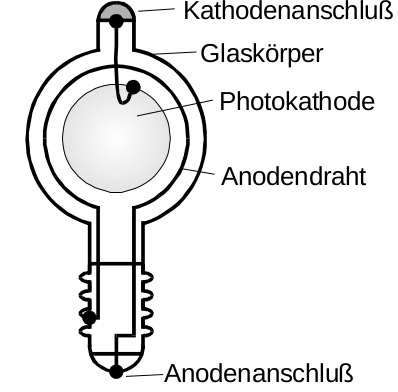
\includegraphics[scale=0.4]{aufbau.png}
  \caption{Schematischer Aufbau der Photozelle.}
  \label{fig:2}
\end{figure}
In Abbildung \ref{fig:2} ist der Aufbau der die im Versuch verwendeten Photozelle
zu sehen. Diese besteht äußerlich aus einem evakuiertem Glaskörper.
Die Kathode wird realisiert durch eine durch eine aufgedampfte Metall oder Legierungsschicht,
die Anode durch einen kreiförmigen Drahtring, der parallel zur Kathode angebracht ist. \\
\\
Um mit monochromatischem, aber verschieden langem Licht zu arbeiten, wird der in Abbildung \ref{fig:3}
\begin{figure}[h]
  \centering
  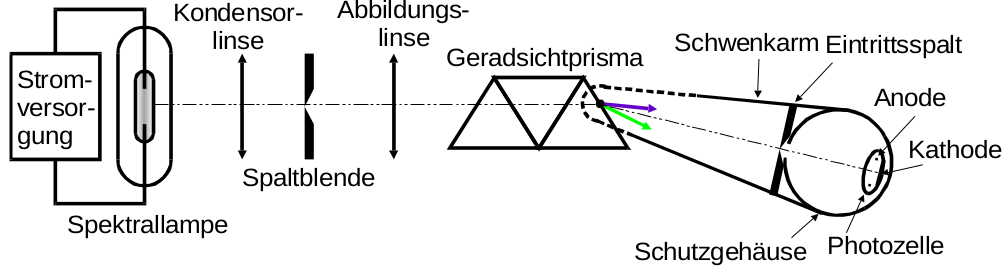
\includegraphics[scale=0.4]{optisch.png}
  \caption{Aufbau zur Aufspaltung des verwendeten Lichts.}
  \label{fig:3}
\end{figure}
dargestellte Aufbau verwendet. Durch Aufspaltung des Lichts am Geradsichtprisma erhält man Spektrallinien,
die monochromatisch sind. Somit wird durch Schwenken des Schutzgehäuses erreicht, dass die Photokathode
mit Licht mit unterschiedlicher Wellenlänge $\lambda$ bestrahlt wird. \\
\\
Um die Energie der ausgelösten Elektronen zu bestimmen, wird das Schaltbild aus Abbildung \ref{fig:4}
verwendet.
\begin{figure}[h]
  \centering
  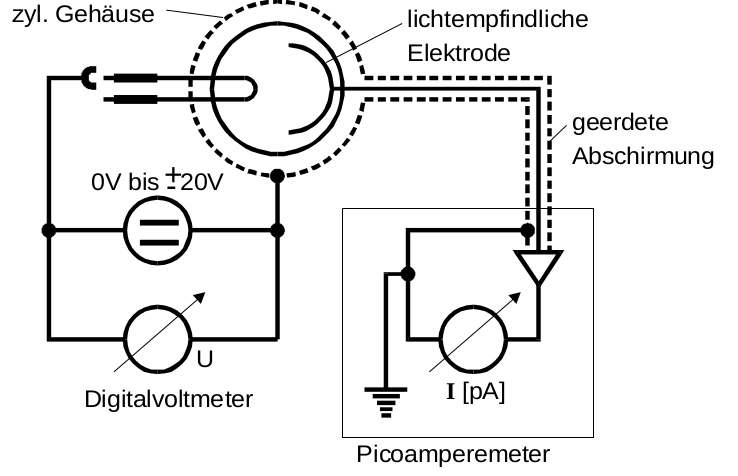
\includegraphics[scale=0.4]{schaltbild.png}
  \caption{Schaltbild zur Untersuchung der Ernergie der ausgelösten Elektronen.}
  \label{fig:4}
\end{figure}
Dies ist die sogennante Gegenfeldmethode. Zwischen Kathode und Anode wird eine variable
Spannung $U$ angelegt, die umpolbar ist. Mit dem Picoamperemeter lässt sich dann der
Photostrom messen.
\subsection{Versuchsdurchführung}
Für fünf verschiedene Wellenlängen wird der Photostrom in Abhängigkeit von der Gegenspannung
$U$ gemessen. Es werden pro Wellenlänge zehn Messwerte aufgenommen. Dabei wird bei besonders
langwelligem Licht teilweise eine Beschleunigerspannung angelegt, um die Grenzspannung
$U_g$ zu erreichen. Danach wird für die Wellenlänge
$\lambda = \SI{578}{\nano\meter}$ eine Kennlinie aufgenommen. Dazu wird die Spannung
im Bereich $\SI{-20}{\volt} \leq U \leq \SI{20}{\volt}$ variiert und dabei der Photostrom
aufgenommen.

\section{Auswertung}

\section{Diskussion}
\newpage
\nocite{*}
\printbibliography
